\documentclass{beamer}
\setbeamertemplate{footline}[frame number] 

\mode<presentation> {
%  \usetheme{Boadilla}
  %\usetheme{Dresden} <-- myabe this one
% \usetheme{Hannover} 
 %\usetheme{Madrid}
 %\usetheme{Malmoe} %like Warsaw but blue
 %\usetheme{Marburg} %dark blue/black gradient on right, white body on left
\usetheme{Montpellier} %blue borders, with tree section structure
  %\usetheme{PaloAlto} %blue bg top and left, white body
  %\usetheme{Pittsburgh} %simple white body
  %\usetheme{Rochester} %simple blue box header and white body
  %\usetheme{Singapore} %cool dots + gradient bg
  %\usetheme{Szeged} %cool dots + box
 %\usetheme{Warsaw}
  \setbeamercovered{transparent}
}

\usepackage[english]{babel}

\usepackage[latin1]{inputenc}

\usepackage{times}
\usepackage[T1]{fontenc}



% adds underlines/strikethroughs
%\usepackage{ulem}

\title[Evaluating the Performance of Network Protocol Processing on Multi-core Systems] % (optional, use only with long paper titles)
{Evaluating the Performance of Network Protocol Processing on Multi-core Systems\\}

\subtitle {AINA 2009} 

\author[] % (optional, use only with lots of authors)
{\textbf{Matthew Faulkner} \and Andrew Brampton \and Stephen Pink}

% - Use the \inst{?} command only if the authors have different
%   affiliation.

\institute[Lancaster University] % (optional, but mostly needed)
{
  Computing Department\\
  Lancaster University\\
  Lancaster\\
}

\date[\today] % (optional)
{
\today
}

\subject{AINA Talk}

\pgfdeclareimage[height=0.7cm]{university-logo}{lancslogo}
\logo{ \pgfuseimage{university-logo} }

% If you wish to uncover everything in a step-wise fashion, uncomment
% the following command:

%\beamerdefaultoverlayspecification{<+->}

% suppresses all navigation symbols
\setbeamertemplate{navigation symbols}{}

\begin{document}
\begin{frame}
  \titlepage
  %\tiny{\SVN $Revision$}
\end{frame}

\begin{frame}
\begin{footnotesize}
\tableofcontents
\end{footnotesize}  
  % You might wish to add the option [pausesections]
\end{frame}

\section{Introduction}
\begin{frame}
  \frametitle{Introduction}
  	This presentation shows a series of experiments that evaluate how many architectures affect network protocol processing. Why?
	\begin{itemize}
		\item Network speeds are increasing, e.g. 10Mbps to 1GbE to 10GbE to 40GbE and 100GbE?
	 	\item Advances in clock speeds of microprocessors is slowing down
	 		\begin{itemize}
	 			\item Transistors are just to small!
	 		\end{itemize}
	 	\item Many core systems are being introduced by the microprocessor architecture as the new way to keep with Moorse Law
	\end{itemize}
\end{frame}

\subsection[Terms]{Terminology}

\begin{frame}
    \frametitle{Terminology}
	Throughout this presentation (and the associated paper) the follow terms are used
	\begin{itemize}
		\item Processor - a single physical entity which includes one or more multiple dies
		\item Die - an integrated circuit upon which at least one core may be placed alongside other components, e.g. cache, bus interface etc
		\item Core - a computational unit with the ability to execute instructions.
	\end{itemize}
\end{frame}

\section{Methodology}

\subsection[Using Multiple Cores]{How to use Multiple Cores}

\begin{frame}
    \frametitle{How can multiple cores be used?}
    Assuming packet level parallelism
	\begin{center}
		\includegraphics[scale=0.7]{../Figures/network_stack.pdf}
	\end{center}
\end{frame}

\subsection[Using Multiple Cores]{What System is Used for the Evaluation}
\begin{frame}
    \frametitle{What System is Used for the Evaluation}
    Two of the following (one client and one server)
	\begin{center}
		\includegraphics[scale=0.4]{../Figures/intelxeondia.pdf}
	\end{center}
	\begin{small}Access Speeds (ns): 
	\begin{itemize}
	\item L1 - 1.5
	\item L2 - 7.1
	\item Main memory - 107.3 (sequential) or 187.8 (non-sequential)
	\end{itemize}\end{small}
\end{frame}

\subsection[Using Multiple Cores]{How are the multiple cores used?}
\begin{frame}
    \frametitle{How are the multiple cores used in this system?}
    This paper identifies four possible scenarios
    \begin{itemize}
    	\item \textbf{Same Core} - Both the network protocol processing and application processing take place on the same core, e.g. core 0
		\item \textbf{Same Die} - Network protocol processing and application processing take place on different cores, albeit they are on the same die, i.e. they share a L2 cache
		\item \textbf{Same Processor} - Network protocol processing and application processing take place on the same processor, i.e. they share the same FSB
		\item \textbf{Same Computer} - Network protocol processing takes place on a core of processor 0 and application processing takes place on a core of processor 1
    \end{itemize}
\end{frame}

\begin{frame}
    \frametitle{How are the multiple cores used in this system? (2)}
  	\begin{table}[tb]
       		 \begin{tabular}{|c|c|c|l|} \hline
                                  & Shared Resources \\ \hline
    	    \textbf{Same Core}        & CPU cycles, both caches, FSB \& Northbridge    \\ \hline
	       	\textbf{Same Die}         & L2 Cache, FSB and Northbridge \\ \hline
    	    \textbf{Same Processor}   & FSB and Northbridge \\ \hline
	        \textbf{Same Computer}    & North bridge  \\ \hline
        	\end{tabular}	
	\end{table}
\end{frame}

\subsection[Using Multiple Cores]{Experimental Details}
\begin{frame}
    \frametitle{Experiential Setups}
	All experiments 
	\begin{itemize}
		\item Used a custom built tool which allowed the application processing affinity to be set
		\item Had a fixed network protocol processing affinity
		\item Setup TCP connection(s) between the client and server on a link with a 1500byte MTU
		\item Sent 1448 byte packets at a specified bit rate
		\item Recorded different metrics using several different tools (see paper for details)
	\end{itemize}
	
\end{frame}

\begin{frame}
    \frametitle{Experiential Setups (2)}
    However, two different setups were used
	\begin{itemize}
		\item Single connection - Two 1GbE were bonded together to form a single 2GbE link
		\item Multiple connections - Four 1GbE nics were placed in each machine and a TCP connection established between each pair
	\end{itemize}
\end{frame}

\section{Results}
\subsection[Single Connection Results]{Single Connection Results}
\begin{frame}
	\frametitle{Goodput and CPU utilisation for the different scenarios}
    \includegraphics[width=0.5\columnwidth]{../Graphs/intel/two_machines/requested_goodput_vs_actual_throughput}
    \includegraphics[width=0.5\columnwidth]{../Graphs/intel/two_machines/requested_goodput_vs_cpu_total}
    \\All scenarios achieve the same rate. However, each scenario uses a different amounts of CPU resources.
     \\The drop in CPU utilisation at around 75MBps is due to Linux's interrupt mitigation API known as NAPI. See the paper for further details.
\end{frame}

%\begin{frame}
%	\frametitle{Goodput and CPU utilisation for the different scenarios}
%    \includegraphics[width=0.5\columnwidth]{../Graphs/intel/two_machines/requested_goodput_vs_actual_throughput}
%    \includegraphics[width=0.5\columnwidth]{../Graphs/intel/two_machines/requested_goodput_vs_cpu_total}
%
%\end{frame}

\begin{frame}
	\frametitle{CPU Caches}
    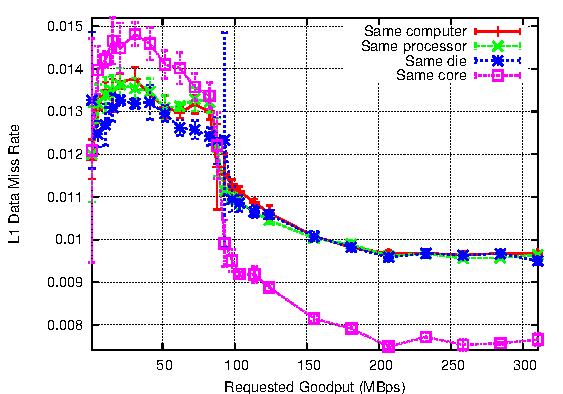
\includegraphics[width=0.5\columnwidth]{../Graphs/intel/two_machines/requested_goodput_vs_L1_MISS_RATE}
    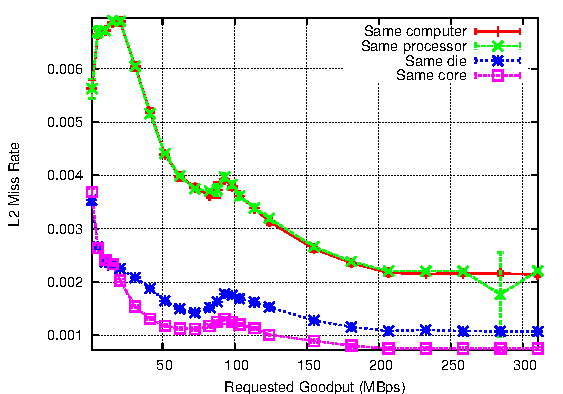
\includegraphics[width=0.5\columnwidth]{../Graphs/intel/two_machines/requested_goodput_vs_L2_MISS_RATE}
    \\The ``Miss Rate'' is the number of cache lines fetched in to that level of cache divided by the number of complete instructions. Thus the higher this rate, the more time is spent fetching from a higher level in the cache hierarchy
\end{frame}

\begin{frame}
	\frametitle{Front Side Bus}
   \begin{center}
		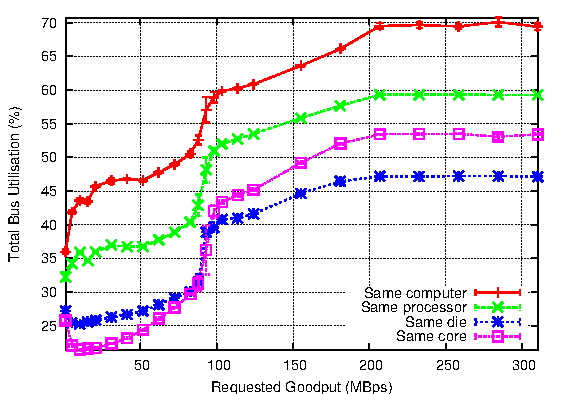
\includegraphics[width=0.5\columnwidth]{../Graphs/intel/two_machines/requested_goodput_vs_BUS_UTIL}
	\end{center} 
    The Northbridge contains a snoop filter which stops adverse traffic going on to the wrong bus

\end{frame}

\subsection[Using Multi-connection]{Multiple Connection Results}

\begin{frame}
	\frametitle{Goodput and CPU utilisation for the different scenarios}
		\includegraphics[width=0.5\columnwidth]{../Graphs/intel/two_machines/4_connections/requested_goodput_vs_actual_throughput}
		\includegraphics[width=0.5\columnwidth]{../Graphs/intel/two_machines/4_connections/requested_goodput_vs_cpu_total}
	\\Now, the scenarios have a different maximum throughput. Same core is limited by raw CPU cycles.
\end{frame}

\begin{frame}
	\frametitle{Multiconnection Experiments}
	General Comments
	\begin{itemize}
		\item Difference in performance of each scenario can be attributed to (a) caches (b) fsb
		\item Performance of the Same Core scenario is 15\% less in these tests
			\begin{itemize}
				\item The network buffer could not be emptied fast enough (see the paper for further details)
			\end{itemize}
	\end{itemize}
\end{frame}


\section{Conclusions}

\subsection[Discussions]{Discussion and Implications on Related Work}
\begin{frame}
	\frametitle{Some General Comments}
	\begin{itemize}
		\item The results can be generalised
			\begin{itemize}
				\item We have done similar studies using a 10GbE NIC and the hardware architecture has the same impact 
			\end{itemize}
		\item Vastly important area of research especially with the introduction of NUMA many core architectures
		\item Analysis could be used along with Receive Side Scaling type technologies
		\item Very useful for Asymmetric Multiprocessors, for example packet processing engines \textit{etc}

	\end{itemize}
\end{frame}


\subsection[Discussions]{Concluding Remarks}
\begin{frame}
	\frametitle{Conclusions}
	\begin{itemize}
		\item Network protocol processing and application processing are affected by the resources they share
		\item A performance decrease of over 40\% occurs if the wrong cores are used
		\item When an application only requires small throughput consider using the same core all processing
		\item When an application requires larger throughput use two cores which share a L2 cache
	\end{itemize}
\end{frame}


\section[Thank You + Questions?]{Thank-you}
\begin{frame}
  \begin{center}
    \alert{\textit{Network architectures now need to consider microprocessor design}}
	 \titlepage
 \end{center}
\end{frame}




\end{document}
